\documentclass{article} % For LaTeX2e
\usepackage{nips15submit_e,times}
\usepackage{hyperref}
\usepackage{url}

% Packages I'm adding in - rclui
\usepackage{graphicx}
\usepackage{subcaption}
%\documentstyle[nips14submit_09,times,art10]{article} % For LaTeX 2.09

\title{GANime Faces - An Undergraduate Study in Generating Anime Faces from an Adversarial Network}

\author{
Ivana Jovasevic\\
Engineering Science\\
Simon Fraser University\\
Burnaby, BC \\
\texttt{ijovasev@sfu.ca} \\
\And
Ryan Lui \\
Engineering Science \\
Simon Fraser University\\
Burnaby, BC \\
\texttt{rclui@sfu.ca} \\
\AND
Sami Ma \\
Computing Science \\
Simon Fraser University\\
Burnaby, BC \\
\texttt{masamim@sfu.ca} \\
\And
Adnan Syed \\
Engineering Science \\
Simon Fraser University\\
Burnaby, BC \\
\texttt{ssyed@sfu.ca} \\
\And
Greyson Wang \\
Engineering Science \\
Simon Fraser University\\
Burnaby, BC \\
\texttt{greysonw@sfu.ca} \\
}

% The \author macro works with any number of authors. There are two commands
% used to separate the names and addresses of multiple authors: \And and \AND.
%
% Using \And between authors leaves it to \LaTeX{} to determine where to break
% the lines. Using \AND forces a linebreak at that point. So, if \LaTeX{}
% puts 3 of 4 authors names on the first line, and the last on the second
% line, try using \AND instead of \And before the third author name.

\newcommand{\fix}{\marginpar{FIX}}
\newcommand{\new}{\marginpar{NEW}}

\nipsfinalcopy % Uncomment for camera-ready version

\begin{document}


\maketitle

\begin{abstract}
This paper explores the use of Generative Adversarial Networks (GANs) to create anime character faces. The research done is based on the Keras-GAN-AnimeFace-Character repository by forcecore \cite{Keras-GAN-Animeface-Character}. After running the default model, we changed various hyperparameters to see its effects on image generation, including batch size, learning rates, and types of optimizers.  We also ran the animeface-character-dataset through different models to observe the output.
\end{abstract}

\section{Introduction}

Machine learning is a vast, constantly growing research area with many different models and approaches for solving problems. In this class we have learned about discriminative models, which are used to model the decision boundary in a classification problem, and generative models, which are used to model the actual distribution of a class, and can generate synthetic example data (ch4 slides p73). The purpose of this paper is to investigate the use of both of these models in a Generative Adversarial Network (GAN).

GANs were first proposed by Ian Goodfellow et al. as “a new framework for estimating generative models via an adversarial process” \cite{paperIanGAN}. The network is comprised of a discriminative model that is trained to classify between ‘real’ training data and ‘fake’ generated data, and a generative model that is trained to generate the data to trick the discriminative model. This method offers a solution to the problem of poorly estimated generative models. By forcing the networks to compete, the generative model is driven to improve its output until the ‘fake’ generated data is indistinguishable from the ‘real’ training data \cite{paperIanGAN}.  Deep Convolutional GANs in particular have been proven to be one of the most successful network designs, utilizing convolutional layers from convolutional neural networks (CNN) that have proved successful in computer vision \cite{unsupDCGAN}. 

In this paper, we will explore the use of a GAN to generate anime character faces. The inspiration for this topic stems from a personal interest in anime, and the availability of the data to train the model. Our paper is based on the model developed by forcecore \cite{Keras-GAN-Animeface-Character} and was trained with data from animeface-character-dataset \cite{animeface-character-dataset}. In this paper, we explore the outputs from the Keras-GAN-AnimeFace-Character model along with other real face GAN models, and discuss a variety of experiments we performed on these models in an attempt to improve the results. 


\section{Approach}
The Keras-GAN-AnimeFace-Character model is a GAN developed using Keras \cite{Keras-GAN-Animeface-Character}. The model is trained on a batch size of 64 using 64 by 64 pixel images. Loss is calculated using the Adam optimizer. Figure \ref{fig:kerasReal} shows some example training images from the animeface-character-dataset, and Figure \ref{fig:kerasGen} and \ref{fig:kerasLoss} show the output of the unmodified model and its loss function, respectively.

\begin{figure}[h!]
	\centering
	\begin{subfigure}[b]{0.24\linewidth}
		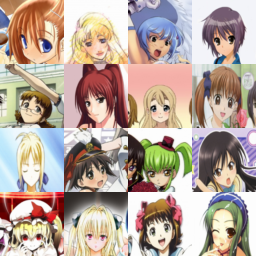
\includegraphics[width=\linewidth]{keras_reals.png}
		\caption{Training Images}
		\label{fig:kerasReal}
	\end{subfigure}
	\begin{subfigure}[b]{0.24\linewidth}
		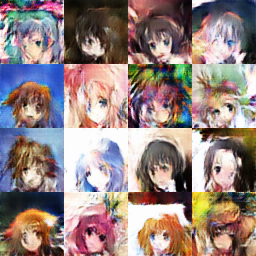
\includegraphics[width=\linewidth]{keras_gen.png}
		\caption{Output at batch 5000}
		\label{fig:kerasGen}
	\end{subfigure}
	\begin{subfigure}[b]{0.5\linewidth}
		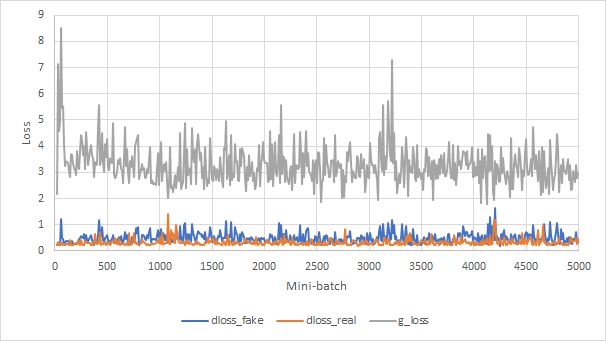
\includegraphics[width=\linewidth]{keras_loss.png}
		\caption{Loss function of discriminator and generator}
		\label{fig:kerasLoss}
	\end{subfigure}
	\caption{Results from running the default Keras-GAN-AnimeFace-Character model.}
	\label{fig:kerasDefault}
\end{figure}

	Our approach for this paper is to perform a set of experiments on the default model and observe the outputs in hopes of improving the results. The attempted experiments are listed below, and discussed in further detail in the Experiments section of the paper: 

\begin{enumerate}
	\item Making simple changes to the default model, such as modifying batch size and flipping label assignments. 
	\item Using a variety of strategies in an attempt to optimize the code, including modifying the learning rates, using the Adam and AdaMax optimizers, and applying Stochastic Gradient Descent (SGD).
	\item Running different models on the animeface-character-dataset to compare results to the original model.
\end{enumerate}

\section{Experiments}

\subsection{Experiment: changing batch size and flipping labels}
After running the Keras-GAN-AnimeFace-Character model unmodified, our first experiment was to make minor changes based on researched tips for training GANs \cite{ganTrainTips}. We ran the model using different batch sizes (16, 32, 64 and 128), to evaluate the significance of how many epochs were necessary to train the model. The results from the smallest and largest batch size run can be seen in Figure \ref{fig:kerasBatchGen} below.

\begin{figure}[h!]
	\centering
	\begin{subfigure}[b]{0.24\linewidth}
		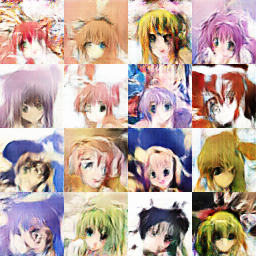
\includegraphics[width=\linewidth]{ijovasev-12-batch-size-16-gen.png}
		\caption{Batch size 16}
		\label{fig:kerasBatch16Gen}
	\end{subfigure}
	\begin{subfigure}[b]{0.24\linewidth}
		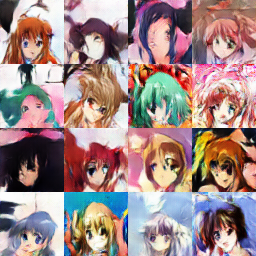
\includegraphics[width=\linewidth]{ijovasev-13-batch-size-128-gen.png}
		\caption{Batch size 128}
		\label{fig:kerasBatch128Gen}
	\end{subfigure}
	\caption{Generated images from running the model with various batch sizes}
	\label{fig:kerasBatchGen}
\end{figure}

\begin{figure}[h!]
	\centering
	\begin{subfigure}[b]{0.49\linewidth}
		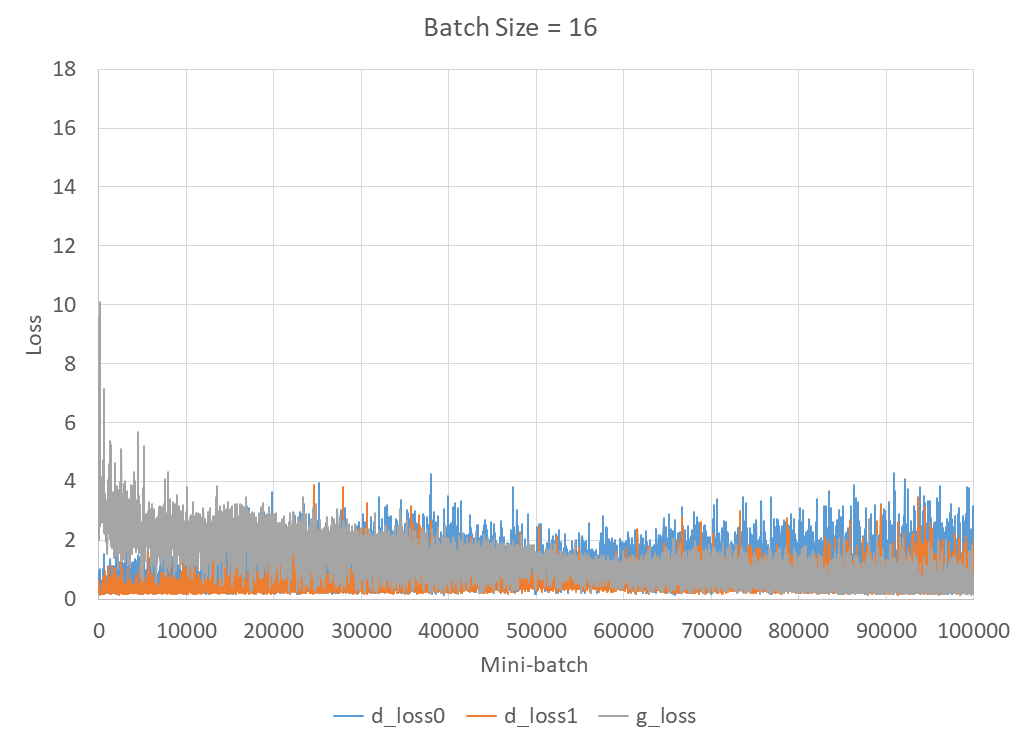
\includegraphics[width=\linewidth]{ijovasev-12-batch-size-16.png}
		\caption{Batch size 16}
		\label{fig:kerasBatchLoss16}
	\end{subfigure}
	\begin{subfigure}[b]{0.49\linewidth}
		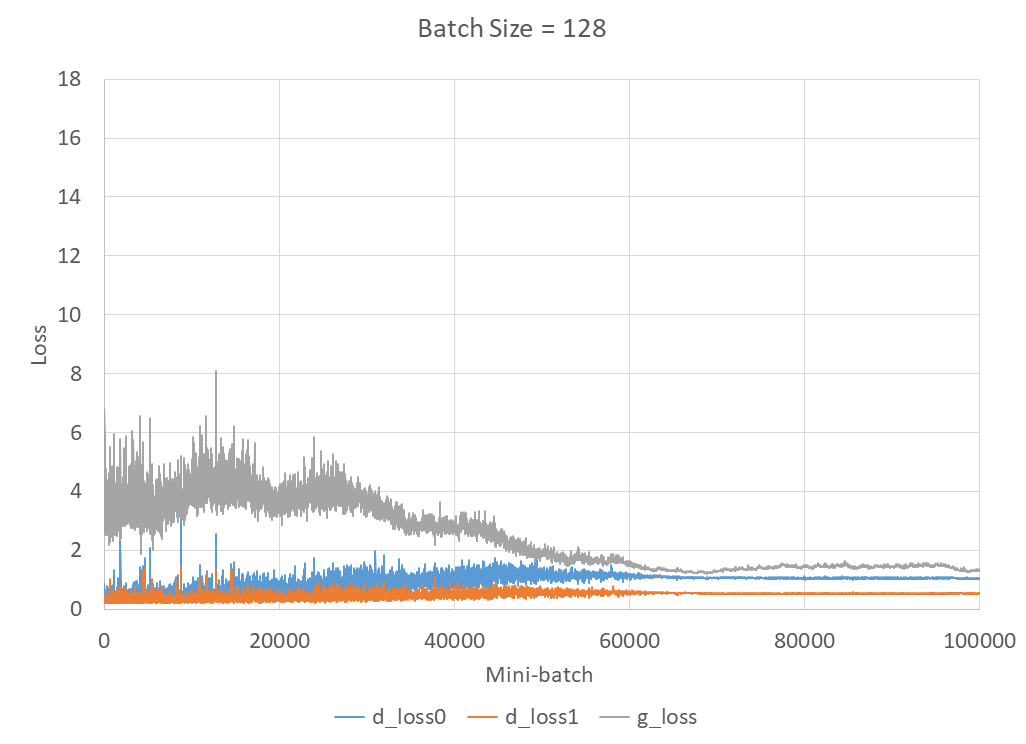
\includegraphics[width=\linewidth]{ijovasev-13-batch-size-128.png}
		\caption{Batch size 128}
		\label{fig:kerasBatchLoss128}
	\end{subfigure}
	\caption{Loss graphs from running the model with various batch sizes}
	\label{fig:kerasBatchLoss}
\end{figure}

By default, the model ran with a batch size of 64. By modifying the batch size, we observed that a smaller batch size of 16 ran much faster, and the resulting images appear to be about as good. On the contrary, running the model with a larger batch size of 128 failed at around 60000 mini-batches, as can be seen in Figure \ref{fig:kerasBatchLoss}, and the resulting images do not appear to have improved.  d\_loss0 indicates the loss of the discriminator when trained with fake images, and d\_loss1 is the loss when trained with real images.

An additional modification we made was flipping the labels for generated and real images, based on the idea that this would help with gradient flow in early iterations of training \cite{ganTrainTips}.

The default labels are soft label where the real would be some number close to 0 and the fake would be some number close to 1. We flipped the labels such that the real images were close to 1 and fake images were close to 0. The idea was that it might help the cases where we might get stuck at a local minimum. With this in mind, we ran the GAN and took a look at the results. The resulting pictures from flipping the labels looked cleaner and more of a face than the default settings. 30,000 was the best of both, but the flipped labels images had eyes that were easily distinguishable. At 100,000, they both looked bad and the images were duplicating because of the overfitting. Even at 100,000, the flipped labels had less noise, less duplicate pictures and still somewhat resembled a face. It seemed like an initial success; however, taking a looking at the loss graph between the two, this was not the case. Overall, the loss of the flipped labels were higher and less stable than the default. We did not get a chance to examine why this was the case; however, something we could have tried is flipping the labels occasionally, rather than all the time, to see if that can negate the effects of the poor loss while retaining the benefits of a cleaner image. 

\begin{figure}[h!]
	\centering
	\begin{subfigure}[b]{0.24\linewidth}
		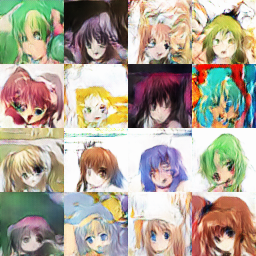
\includegraphics[width=\linewidth]{syed-default-30k.png}
		\caption{Default at 30,000}
		\label{fig:kerasLabelsDefault30k}
	\end{subfigure}
	\begin{subfigure}[b]{0.24\linewidth}
		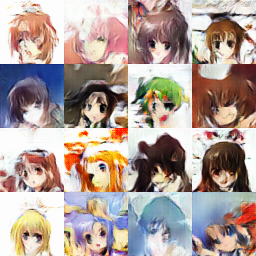
\includegraphics[width=\linewidth]{syed-flipped-30k.png}
		\caption{Flipped at 30,000}
		\label{fig:kerasLabelsFlipped30k}
	\end{subfigure}
	\begin{subfigure}[b]{0.24\linewidth}
		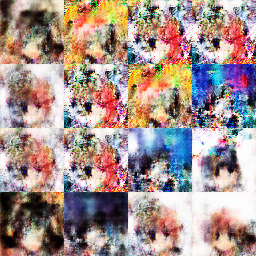
\includegraphics[width=\linewidth]{syed-default-100k.png}
		\caption{Default at 100,000}
		\label{fig:kerasLabelsDefault100k}
	\end{subfigure}
	\begin{subfigure}[b]{0.24\linewidth}
		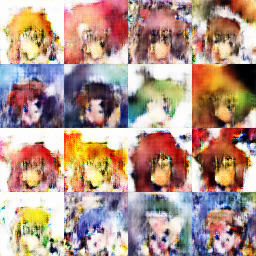
\includegraphics[width=\linewidth]{syed-flipped-100k.png}
		\caption{Flipped at 100,000}
		\label{fig:kerasLabelsFlipped100k}
	\end{subfigure}
	\caption{Generated images at various mini-batches with and without flipped classifiers}
	\label{fig:kerasLabelsGen}
\end{figure}

\begin{figure}[h!]
	\centering
	\begin{subfigure}[b]{0.49\linewidth}
		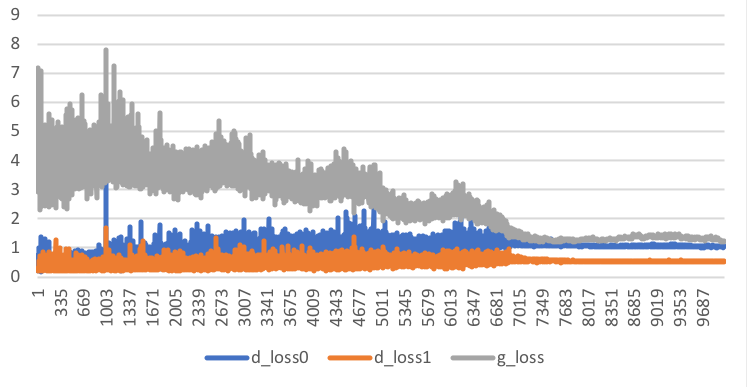
\includegraphics[width=\linewidth]{syed-default-loss.png}
		\caption{Default model}
		\label{fig:kerasLabelsFlippedLoss100k}
	\end{subfigure}
	\begin{subfigure}[b]{0.49\linewidth}
		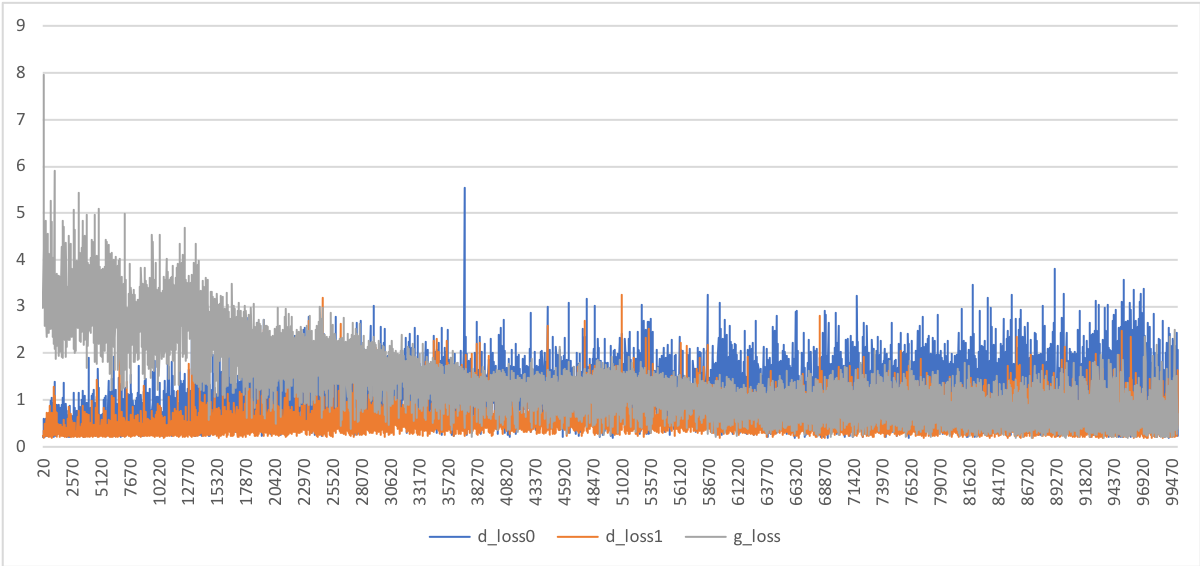
\includegraphics[width=\linewidth]{syed-flipped-loss.png}
		\caption{Flipped labels model}
		\label{fig:kerasLabelsDefaultLoss30k}
	\end{subfigure}
	\caption{Loss graphs from running the model with and without flipped classifiers}
	\label{fig:kerasLabelsGen}
\end{figure}

\subsection{Experiment: changing optimizers and their learning rates}

Some of the other modifications we made included using different optimizers, as suggested by Soumith et al \cite{ganhacks}.  In the default model run, we noticed that the learning began to fail after 70,000 mini-batches, with the generator beginning to generate extremely noisy images.  Adam was the default optimizer that was used, and as such, we first opted to try different values for the discriminator learning rate.  In our first attempt, we made the discriminator learning rate larger, from 0.0002 to 0.001, while keeping all other parameters constant.  This change eliminated the failure we saw.  We believe that the having the learning rate too small for the discriminator made it easier for the generator to “outsmart” the discriminator.  Figure \ref{fig:kerasAdam02} outlines the results.

\begin{figure}[h!]
	\centering
	\begin{subfigure}[b]{0.5\linewidth}
		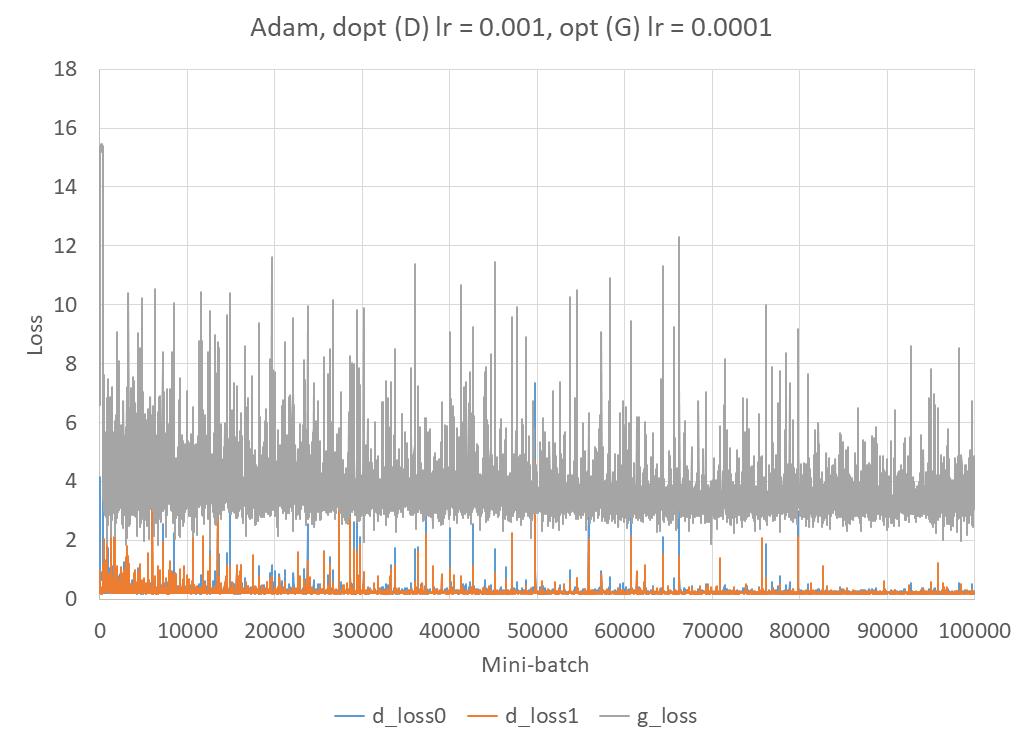
\includegraphics[width=\linewidth]{rclui-02-Adam-dopt-0-001-opt-0-0001.png}
		\caption{Loss}
		\label{fig:kerasAdam02Loss}
	\end{subfigure}
	\begin{subfigure}[b]{0.35\linewidth}
		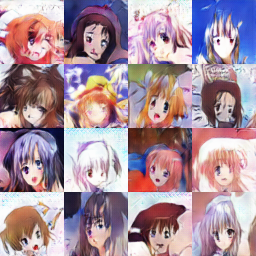
\includegraphics[width=\linewidth]{rclui-02-Adam-gen.png}
		\caption{Generated Image}
		\label{fig:kerasAdam02Gen}
	\end{subfigure}
	\caption{Results from running the model using the Adam optimizer}
	\label{fig:kerasAdam02}
\end{figure}

Next, we modified the generator layers to use 2D upsampling followed by 2D convolution in place of the current 2D transposed convolution from the original model.  2D transposed convolution was noted to exhibit artifacts in the images \cite{conv2dArtifacts} so by forcing upsampling before convolution, we hoped that this would reduce the noise in the generator at 70,000 mini-batches.  This proved to be true, and the losses for both generator and discriminator continually fluctuated.

We also tried using AdaMax and standard stochastic gradient descent, both of which did not succeed.  In the first case, we modified the GAN to use the AdaMax optimizer with various values for the learning rate, but the resulting generated images had noticeably more artifacts.  This was reflected in the loss graph as shown in Figure \ref{fig:kerasAdamax07}.  In the stochastic gradient descent case, we opted to change the discriminator to SGD while keeping the generator on the Adam optimizer.  This led to an early failure, where the generator loss was lower than that of the discriminator, and it was reflected with garbage images.

\begin{figure}[h!]
	\centering
	\begin{subfigure}[b]{0.5\linewidth}
		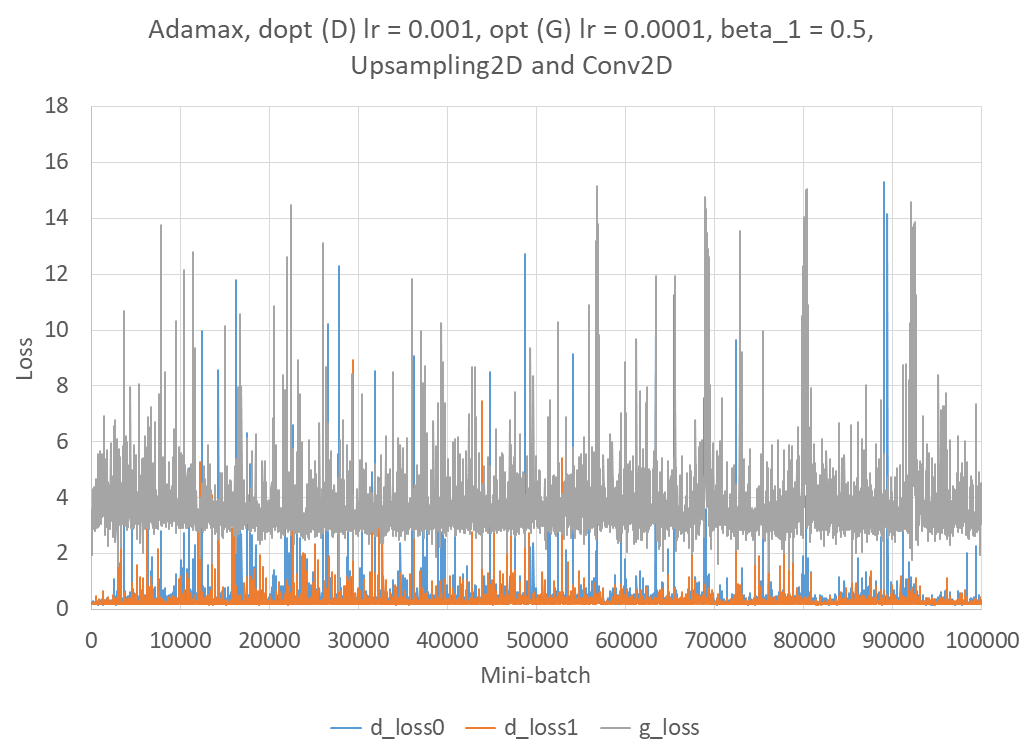
\includegraphics[width=\linewidth]{rclui-07-Adamax.png}
		\caption{Loss}
		\label{fig:kerasAdamax07Loss}
	\end{subfigure}
	\begin{subfigure}[b]{0.35\linewidth}
		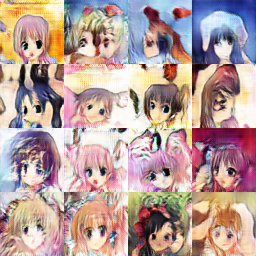
\includegraphics[width=\linewidth]{rclui-07-Adamax-gen.png}
		\caption{Generated Image}
		\label{fig:kerasAdamax07Gen}
	\end{subfigure}
	\caption{Results from running the model using the AdaMax optimizer}
	\label{fig:kerasAdamax07}
\end{figure}

\subsection{Experiment: changing the model - BEGAN}
Our final set of experiments were to change the model we were using, and observe the output for the same animeface-character-dataset.

We considered that anime faces are similar to real faces, and there would be more work done on real face GANs, so we decided to search for repositories on them. One repository is a TensorFlow implementation based on a paper about Boundary Equilibrium Generative Adversarial Networks (BEGAN) \cite{kimBEGAN}. It focused on balancing the generator and discriminator and did not pretrain the discriminator \cite{paperBEGAN}. Using the same 14,000 image dataset (animeface-character-dataset), the images had to be resized to 128x128 with black bar fillings in order to feed them into the network. Preliminary training using the default parameters of the repository led to seemingly overfitting from the generator side. The generator loss was continuously lower than the discriminator loss, and the generated images had repeated faces. The training progressively got worse, where it was stopped at 199,500 mini-batches (Batch size 16) with the result shown in Figure \ref{fig:beganGen199k}.

%\begin{figure}[h!]
%	\centering
%	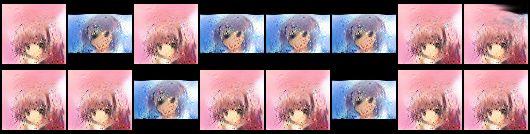
\includegraphics[width=0.7\linewidth]{sami-199500_G.png}
%	\caption{Generated image at 199,500 mini-batches}
%	\label{fig:beganGen199k}
%\end{figure}

The faces generated looked like an anime face, but it is hard to say they are good.  In addition, the overfitting prevents further training. We noticed that the fake and real images that the discriminator uses for training are both blurred, probably to keep the discriminator from overpowering the generator too much. The overall problems could be that the parameters need tuning or that the entire architecture of balancing the networks works against itself.

To prevent overfitting, we tried changing the learning rates (LR) of the networks. The original learning rates were both 8e-5. We lowered the generator LR to 1e-6 and the discriminator LR to 4e-5 in the hopes that the discriminator would learn faster than the generator. The batch size was also lowered to 4 to speed up training. Lowering the LRs in this way ended in failure as the generated faces started with something that could be faces to just blobs, as seen in Figure \ref{fig:beganGen69k}

\begin{figure}[h!]
	\begin{minipage}{0.49\linewidth}
		\centering
		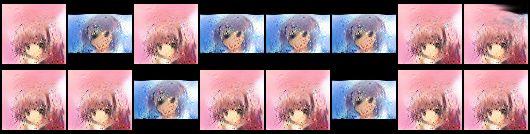
\includegraphics[width=0.95\linewidth]{sami-199500_G.png}	
		\caption{Image at batch 199,500}
		\label{fig:beganGen199k}
	\end{minipage}
	\begin{minipage}{0.49\linewidth}
		\centering
		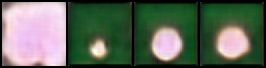
\includegraphics[width=0.95\linewidth]{sami-69000_G.png}
		\caption{Image at batch 69,000}
		\label{fig:beganGen69k}
	\end{minipage}
\end{figure}

The generator loss was still constantly below the discriminator, making the generator still overpowering and overfitting the discriminator.

The next experiment was to keep the LRs the same but slightly lower at 4e-5 as suggested by one of the repository issues \cite{kimBEGAN-30}. The results may have been slightly better, but the same overfitting problem occured.  The generator loss is still below the discriminator loss as seen in Figure \ref{fig:began4e-5}.

\begin{figure}[h!]
	\centering
	\begin{subfigure}[b]{0.6\linewidth}
		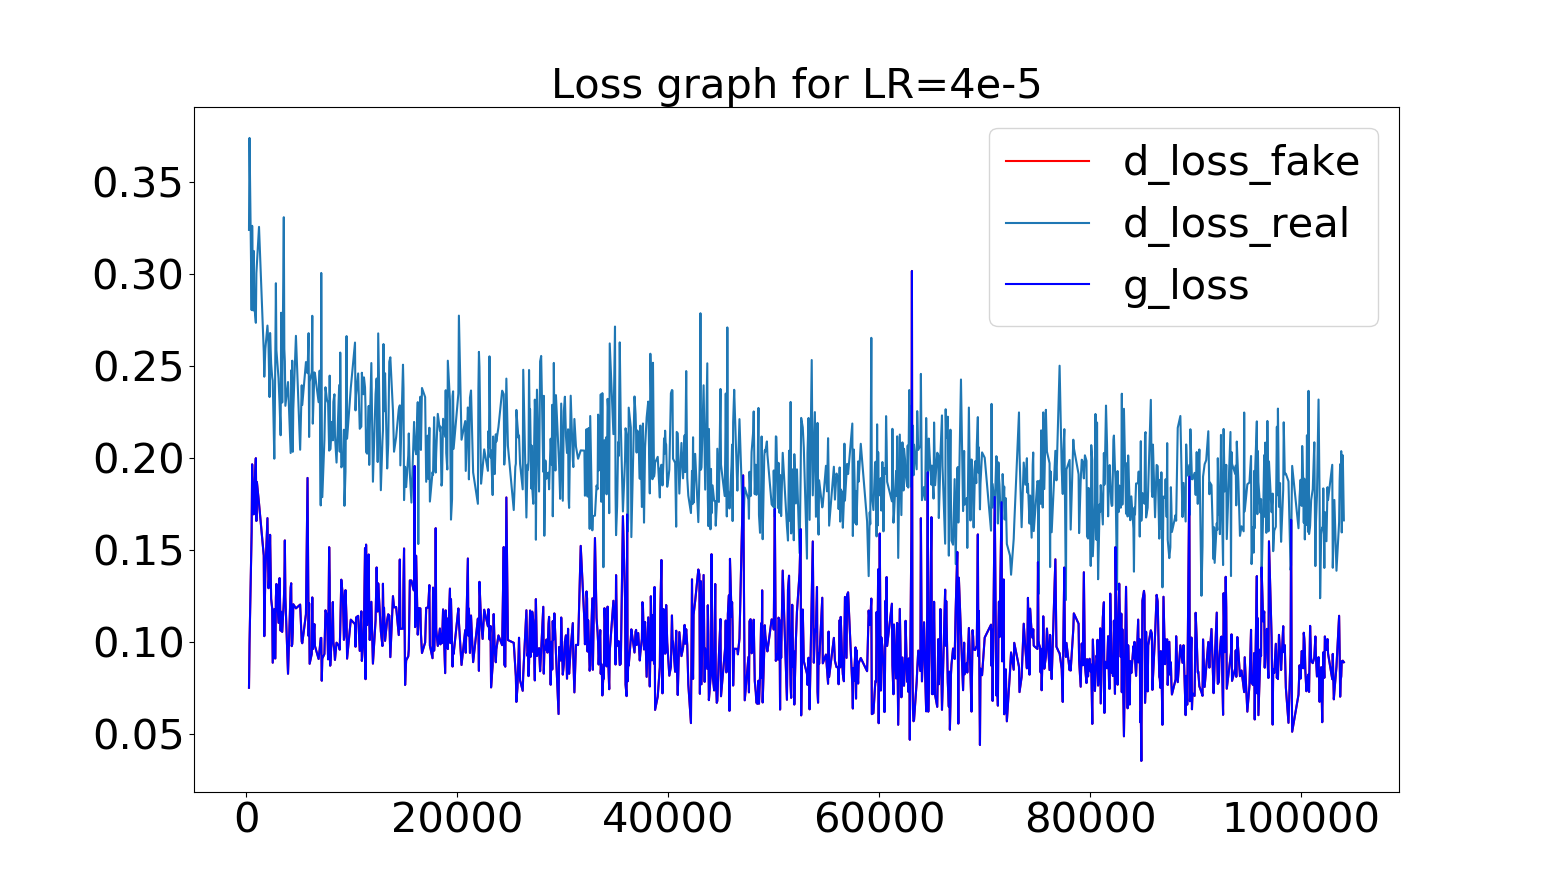
\includegraphics[width=\linewidth]{sami-4e-5-loss.png}
		\caption{Loss}
		\label{fig:began4e-5Loss}
	\end{subfigure}
	\begin{subfigure}[b]{0.39\linewidth}
		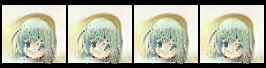
\includegraphics[width=\linewidth]{sami-4e-5-105500_G.png}
		\caption{Generated Image}
		\label{fig:began4e-5Gen}
	\end{subfigure}
	\caption{Results from running the BEGAN model with LR = 4e-5}
	\label{fig:began4e-5}
\end{figure}

More time would need to be allocated to investigate the overfitting problem. This GAN has the potential to create good anime faces. The problem is that the main part of BEGAN is balancing the two networks, which could work against it when one network, namely the generator, is already incredibly overpowering the other.

\subsection{Experiment: Regularization and limiting training}

In this section, we expand on the experiments done with Deep Convolutional Generative Adversarial Networks by Taehoon Kim \cite{kimDCGAN}, who modified the original concept by updating the generator network twice for every discriminator update in order to avoid fast convergence. While this initially produced good results after 50 epochs, by 100 epochs the generator was producing much worse images and the loss value of the discriminator rapidly converged towards zero.

Our first approach was to stop training the discriminator network when its loss value is much smaller than the generator loss, with the goal of allowing the generator to catch up.  We found that stopping training when the ratio of the loss is greater than 10x produced results that were significantly better until 200 epochs. A difference much smaller and much larger than 10x caused the generator to simply produce mostly identical images, as shown in Figure \ref{fig:dcgan} below.

\begin{figure}[h!]
	\begin{minipage}{0.49\linewidth}
		\centering
		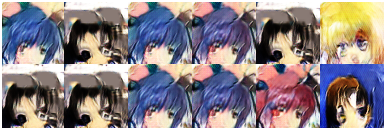
\includegraphics[width=0.95\linewidth]{greyson-dcgan.png}
		\caption{Identical images from DCGAN} %Caption for greyson
		\label{fig:dcgan}
	\end{minipage}
	\begin{minipage}{0.49\linewidth}
		\centering
		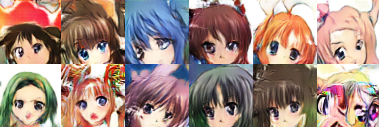
\includegraphics[width=0.95\linewidth]{greyson-dcgan-best.png}
		\caption{Best output from DCGAN} %Caption for greyson
		\label{fig:dcgan-best}
	\end{minipage}

\end{figure}

Combining the original method of updating the generator twice and our method produced comparable results until 160 epoches, but it unfortunately caused the generator to produce mainly identical images afterwards.

Applying L2 regularization had no noticeable effect on the results when applied to the original implementation of the DCGAN. However, when applied to our modified DCGAN, this also caused the generator to continuously produce mainly identical images.

\section{Conclusion}
The purpose of this paper was to research the use of GANs to generate anime character faces. By basing our findings off of a pre-existing model, we were able to observe which modifications and optimizations we could make to improve the generated anime images. We investigated further by running the same dataset through Real Face GAN models, and were able to produce some definitive character faces using these. This project allowed us to become familiar with the inner workings of Generative Adversarial Networks, and explore their capabilities for image generation.  Applications of such networks could potentially be in manga drawing, such as lessening the workload of artists, or providing a starting base in the form of "idea generation".

\section{Contributions}
\begin{enumerate}
	\item Adnan Syed was in charge of researching various tips and tricks to improve how GANs run, and these were implemented and documented by himself and Ivana Jovasevic.
	\item Ryan Lui was in charge of running various optimizations on the Keras model and observing the changes.
	\item Greyson Wang and Sami Ma ran the animeface-character-dataset through Real Face GAN models and researched these results in comparison to the Keras-GAN-AnimeFace-Character model.
	\item Ivana Jovasevic and Ryan Lui were responsible for formatting and finalizing this paper.
\end{enumerate}

\bibliographystyle{unsrt}
\bibliography{bibtex}

\end{document}
